\begin{figure}
\centering
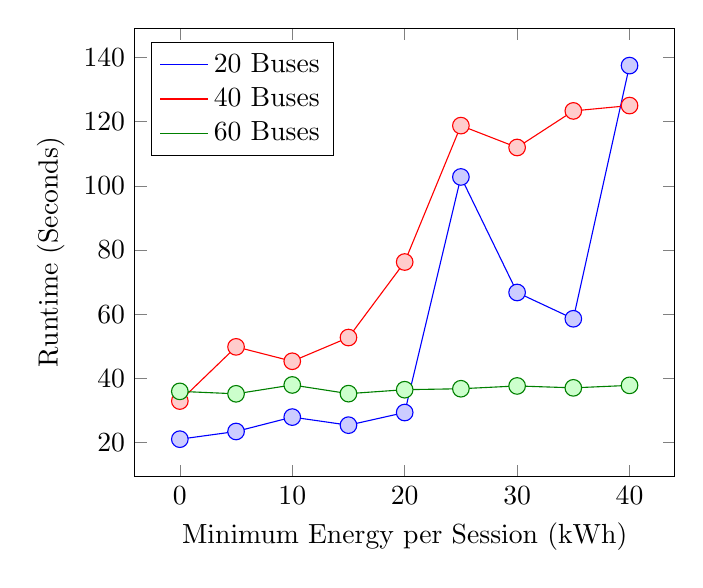
\begin{tikzpicture}
\begin{axis}[xlabel=Minimum Energy per Session (kWh), ylabel=Runtime (Seconds), legend pos=north west]
	\addplot[blue] coordinates {
		(0, 21.00)
		(5, 23.40)
	  (10,27.89)
		(15,25.37)
		(20,29.31)
		(25,102.78)
		(30,66.75)
		(35,58.55)
		(40,137.51)}; 
\addplot[red] coordinates {
		(0, 32.89)
		(5, 49.79)
	  (10,45.30)
		(15,52.70)
		(20,76.25)
		(25,118.79)
		(30,111.97)
		(35,123.37)
		(40,125.04)}; 
\addplot[green!50!black] coordinates {
		(0, 35.91)
		(5, 35.15)
	  (10,37.91)
		(15,35.20)
		(20,36.43)
		(25,36.73)
		(30,37.60)
		(35,37.01)
		(40,37.78)}; 
\addplot[blue!20, draw=blue, only marks, mark size=3pt] coordinates {
		(0, 21.00)
		(5, 23.40)
	  (10,27.89)
		(15,25.37)
		(20,29.31)
		(25,102.78)
		(30,66.75)
		(35,58.55)
		(40,137.51)}; 
\addplot[red!20, draw=red, only marks, mark size=3pt] coordinates {
		(0, 32.89)
		(5, 49.79)
	  (10,45.30)
		(15,52.70)
		(20,76.25)
		(25,118.79)
		(30,111.97)
		(35,123.37)
		(40,125.04)}; 
\addplot[green!20, draw=green!50!black, only marks, mark size=3pt] coordinates {
		(0, 35.91)
		(5, 35.15)
	  (10,37.91)
		(15,35.20)
		(20,36.43)
		(25,36.73)
		(30,37.60)
		(35,37.01)
		(40,37.78)}; 
\legend{20 Buses, 40 Buses, 60 Buses}		
\end{axis}
\end{tikzpicture}
\caption{Comparison of runtime for the uncontested and contested scenarios over different de-fragmentation criteria}
\label{fig:results:defragmentationTimeProTime}
\end{figure}
